\documentclass[11pt]{article}
\usepackage[a4paper,margin=2.3cm]{geometry}
\usepackage[T1]{fontenc}
\usepackage[utf8]{inputenc}
\usepackage{lmodern}
\usepackage{microtype}
\usepackage{amsmath,amssymb}
\usepackage{booktabs}
\usepackage{graphicx}
\usepackage{xcolor}
\usepackage{pgfplots}
\pgfplotsset{compat=1.18}
\usepackage[numbers,sort&compress]{natbib}
\usepackage[hidelinks]{hyperref}
\usepackage{caption}
\captionsetup{font=small,labelfont=bf}

\newcommand{\NR}{\mathrm{NR}_{20}}
\newcommand{\pp}{\,pp}

\title{\textbf{Simple topology does most of the work:\\ a pre-registered evaluation of label-free triage for critical failures in coronary CTA segmentation}}
\author{Maadhav V H\\[2pt]
\small KPR Institute of Engineering and Technology, Coimbatore, India}
\date{November 2026}

\begin{document}
\maketitle

\begin{abstract}
Automated coronary artery segmentation from CT angiography (CCTA) can fail in ways that matter clinically, such as a missed proximal vessel, a broken trunk or a leak into a vein, while still achieving high Dice. We study \emph{label-free review triage}: ranking reconstructions so that a fixed review budget of 20\% of scans catches as many anatomically critical failures as possible, without ground truth at deployment. We defined a reference-based taxonomy of critical failures, pre-registered an analysis plan with success criteria, selected a single model on development data (a stacked logistic model over mask-derived graph, ostium and shape-plausibility features), and evaluated it once on a sealed test set of 160 patients (ImageCAS-X) segmented by a held-out segmenter. The frozen model reached a normalised recall of 0.906 at the 20\% budget (pass), catching 29 of 64 critical reconstructions with precision 0.91, and met the pre-registered comparison with ensemble-agreement quality control. Its advantage over the best pre-specified single-feature rule was +12.5\pp\ (95\% CI $-0.3$ to $+23.9$), missing the pre-registered superiority criterion. In pre-registered follow-up analyses, the advantage replicated across five nnU-Net folds (+11.4\pp, 95\% CI $+3.0$ to $+20.7$; same patients), but shrank or vanished when the input CTs were degraded, and an exploratory fragmentation feature matched the model. We conclude that simple, anatomy-aware topology features capture most of the achievable triage value; a learned combination adds a small, directionally consistent but fragile increment. We report all criteria, negative findings (synthetic-corruption learning, second-annotator relabelling, reduced-order FFR) and the full pre-registration trail.
\end{abstract}

\section{Introduction}
Coronary CCTA segmentation is the first step of many downstream analyses: stenosis grading, plaque quantification and simulated fractional flow reserve. Segmentation models are usually evaluated with volumetric overlap, but overlap is a poor proxy for the failures that change clinical conclusions. A reconstruction can reach Dice $\geq 0.90$ while losing a proximal segment of the left anterior descending artery or bridging the left and right trees (Fig.~\ref{fig:dice}). In deployment there is no ground truth, so such failures must be found by a reviewer, and review time is limited.

We frame quality control as \emph{fixed-budget triage}: given a batch of reconstructions, rank them so that reviewing the top 20\% catches as many \emph{critical} failures as possible. Prior work on segmentation failure detection has benchmarked uncertainty and agreement-based scores across organs \citep{zenk2025failure,kahl2024values} and predicted segmentation quality without ground truth \citep{valindria2017rca,robinson2019qc}. Zenk et al.\ found that simple pairwise agreement within an ensemble is a strong baseline \citep{zenk2025failure}. Coronary trees add a specific difficulty: what matters is connectivity and calibre of a few major vessels, not global overlap \citep{hampe2024gnn}.

Our contributions are:
\begin{enumerate}
\item A reference-based, physically specified taxonomy of \emph{critical} coronary segmentation failures, and a fixed-budget triage protocol with oracle-normalised recall.
\item A pre-registered, sealed evaluation of a label-free triage model on a segmenter it never saw, with pre-specified success criteria reported whether met or not.
\item Pre-registered follow-up analyses: replication across nnU-Net folds, an acquisition-shift stress test, an independent-reference burden analysis and estimator diagnostics. We also report negative findings.
\end{enumerate}
The headline is deliberately modest. A learned model does rank failures well, but most of its value is already available from one or two topology features.

\begin{figure}[t]
\centering
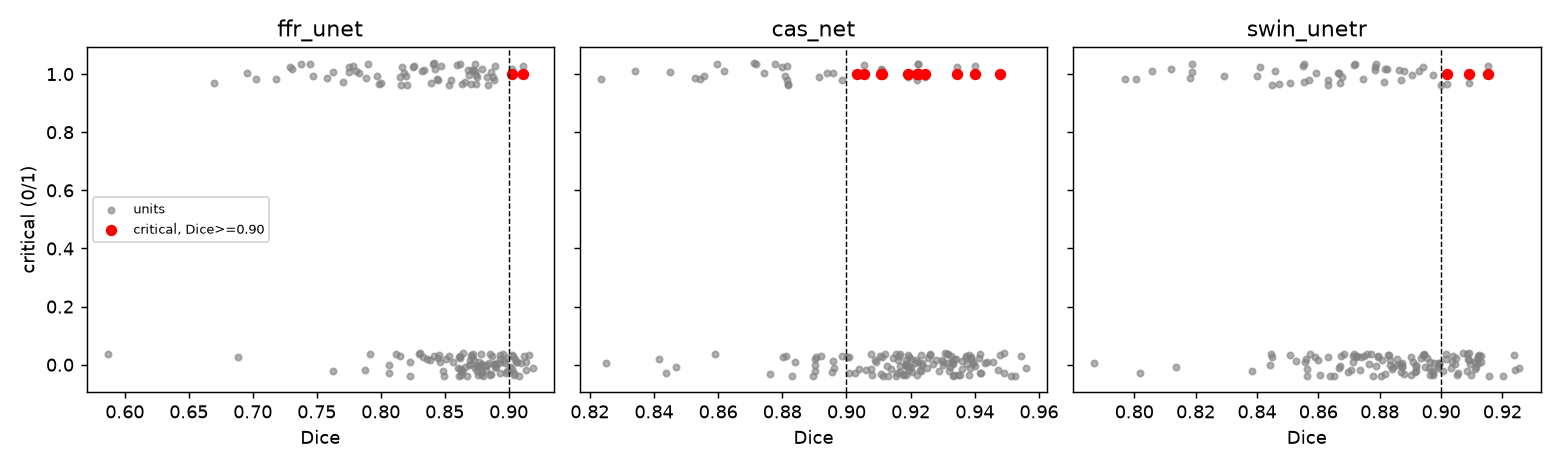
\includegraphics[width=\linewidth]{figures/dice_hides_it.png}
\caption{Dice hides critical failures. Each point is one test reconstruction (160 patients per segmenter); the vertical axis is the binary critical-failure label (jittered). Red points are critical failures with Dice $\geq 0.90$: 2 for FFR-UNet, 12 for CAS-Net and 3 for Swin UNETR.}
\label{fig:dice}
\end{figure}

\section{Data and failure definition}
\paragraph{Data.} We used ImageCAS \citep{zeng2023imagecas}, a public set of 1000 CCTA scans, with the ImageCAS-X re-annotation \citep{bransby2026imagecasx}, which provides 14-class coronary segment labels and centerlines for 800 scans. We used the ImageCAS-X split: 560 training, 80 validation and 160 test patients. No images or labels are redistributed.

\paragraph{Segmenters.} All reconstructions came from the segmentation models released with ImageCAS-X \citep{bransby2026imagecasx}: CAS-Net, Swin UNETR \citep{hatamizadeh2022swinunetr}, FFR-UNet, and a five-fold nnU-Net \citep{isensee2021nnunet} (individual folds and their majority vote). We audited the nnU-Net data preparation: the 160 test scans were never in nnU-Net training. FFR-UNet was used only as a checkpoint released with the dataset; we did not locate a separate primary publication for it.

\paragraph{Critical-failure taxonomy (v3).} Failures are defined against the reference mask and its centerline. A point on the reference centerline is \emph{uncovered} if the nearest predicted lumen voxel is farther than $\max(1.5\,\mathrm{mm}, r)$, where $r$ is the local reference radius. A contiguous uncovered run $\geq 10$\,mm is a missed or broken segment (F1); a reference component split across predicted components is a disconnection (F2); predicted skeleton runs $\geq 10$\,mm lying $> 2$\,mm from the reference lumen are classified as over-extension, halo, detached false positive or leak (F3). A unit (segmenter $\times$ patient) is \textbf{critical} if it has (a) a missed or disconnected left main, LAD, LCx or RCA segment that starts within 50\,mm (geodesic) of the ostium or has reference radius $\geq 1.25$\,mm; (b) a leak (connected run with mean radius $\geq 2$\,mm) or a left--right bridge; or (c) a detached false positive with radius $\geq 2$\,mm. Side branches, posterior descending and posterolateral branches are excluded from (a). The taxonomy was frozen before any QA model was scored. The critical tier was motivated by failure-label prevalence on CAS-Net and Swin UNETR reconstructions (a broader ``severe'' tier fired on 64\% of units, mostly distal branches); FFR-UNet test labels were sealed until the single evaluation. No clinician defined or adjudicated the taxonomy.

\section{Methods}
\paragraph{Triage endpoint.} For each segmenter separately, units are ranked by a score and the top $k = \lfloor 0.2\,n \rfloor$ are reviewed ($k = 32$ of 160). With $P$ critical units and $C$ of them in the reviewed set, recall is $C/P$, precision is $C/k$, and the oracle recall is $\min(P,k)/P$. The primary endpoint is \emph{normalised recall} $\NR = (C/P)/(\min(P,k)/P) = C/\min(P,k)$, with ties at the cut-off averaged. We also report AUROC, the area under the risk--coverage curve (AURC) \citep{geifman2017selective} and raw counts.

\paragraph{Development data and candidate models.} Model fitting and selection used only development data: the 80 validation patients $\times$ \{CAS-Net, Swin UNETR\} (160 units, 21 critical), plus synthetic corruptions of the 560 training reference trees. All candidates use only the predicted mask and, for ostium features, an aorta mask from TotalSegmentator \citep{wasserthal2023totalseg} run on the CT:
\begin{itemize}
\item \textbf{M1, graph features} (14): numbers of components and of components $\geq 10$\,mm, total and per-component skeleton length, share of skeleton length in the two largest components, endpoints, junctions, branch depth, radius violations, tortuosity, maximum radius, leak fraction and gaps.
\item \textbf{M3, ostium features} (7): number and position of ostia, left and right attachment to the aorta, and the length and share of skeleton not attached to an ostium.
\item \textbf{M4, shape plausibility}: a small 3D CNN reading only the binary lumen mask (resampled to $96^3$ at 2\,mm) and trained on synthetic corruptions of training reference trees. The corruption operators were segment deletion, gaps, distal truncation, detached tubes and blobs, leak bulges, left--right bridges and local erosion, plus mild ``clean'' operators. Corruption labels came from the frozen taxonomy.
\end{itemize}
Further candidates (test-time augmentation uncertainty, image-evidence path features and proximal-connectivity features) were evaluated on development data and not selected. The pre-registered selection rule (normalised recall plus AURC, 5-fold patient-grouped cross-validation) selected \textbf{M1+M3+M4}: an L2-regularised logistic model over 22 standardised inputs (development $\NR$ 0.571). The weights, preprocessing and CNN were frozen with SHA-256 hashes before the test evaluation.

\paragraph{Comparators.} (i) The best \emph{pre-specified simple rule}, chosen on development data from four candidates (number of components $\geq 10$\,mm, number of gaps, total-length z-score, maximum-radius z-score): the component count (development $\NR$ 0.476). (ii) Ensemble agreement following \citet{zenk2025failure}: mean pairwise Dice, clDice and Betti-0 error across the five nnU-Net folds, ranking the majority-vote reconstruction. (iii) Random ranking.

\paragraph{Pre-registered success criteria.} The primary evaluation is the single sealed run on FFR-UNet reconstructions of the 160 test patients. \textbf{S1}: $\NR \geq 0.75$. \textbf{S2}: model minus best rule $\geq +10$\pp\ $\NR$ with the paired patient-bootstrap 95\% CI (2000 resamples) excluding 0. \textbf{S3}: non-inferior to the best ensemble comparator (difference $\geq -5$\pp). \textbf{S4}: recall of critical units with Dice $\geq 0.90$ at least 50\%. \textbf{S5}: segment localisation, which was not implemented. A leave-one-segmenter-out (LOSO) analysis over \{CAS-Net, Swin UNETR, FFR-UNet\} was pre-specified as secondary.

\paragraph{Pre-registration trail.} The analysis plan and eight dated addenda (A--H, ending with the freeze) were written before the test evaluation. After it, six further dated addenda (I--N) with ten errata were written before each follow-up analysis was computed; each follow-up was run once on the sealed outputs. All documents are kept with commit history in the project repository. This is a self-maintained record, not a public registry, and we treat it as such.

\section{Results}
\subsection{Primary sealed evaluation}
Table~\ref{tab:main} summarises the sealed evaluation. On FFR-UNet, the held-out segmenter, 64 of 160 reconstructions (40\%) were critical. Reviewing 32, the frozen model caught 29 (precision 0.91, raw recall 0.45; the oracle could catch 32). The pre-specified rule caught 25.

\begin{table}[t]
\centering
\small
\caption{Sealed test evaluation (160 patients per segmenter). $P$: critical units. $\NR$: normalised recall at the 20\% budget. CIs are paired patient bootstrap 95\%. FFR-UNet is the pre-registered primary and was never used in development; CAS-Net and Swin UNETR validation (not test) reconstructions were development data; nnU-Net reconstructions were never used for fitting.}
\label{tab:main}
\begin{tabular}{lrrrrl}
\toprule
Reconstructions & $P$ & $\NR$ model & $\NR$ rule & AUROC model & $\Delta\NR$ (model $-$ rule) \\
\midrule
FFR-UNet (primary) & 64 & 0.906 & 0.781 & 0.845 & $+0.125$ $[-0.003,\,+0.239]$ \\
CAS-Net & 34 & 0.625 & 0.523 & 0.813 & $+0.102$ $[-0.034,\,+0.225]$ \\
Swin UNETR & 45 & 0.719 & 0.556 & 0.810 & $+0.163$ $[+0.032,\,+0.318]$ \\
nnU-Net majority vote & 30 & 0.600 & 0.420 & 0.814 & $+0.180$ \\
\bottomrule
\end{tabular}
\end{table}

\paragraph{Criteria.} \textbf{S1 passed} ($\NR$ 0.906 $\geq$ 0.75). \textbf{S2 failed}: the gain over the rule was $+12.5$\pp, above the $+10$\pp\ bar, but the 95\% CI was $[-0.3, +23.9]$\pp. The AUROC difference was positive ($+0.064$ $[+0.007, +0.119]$). \textbf{S3 passed}: the best ensemble comparator (pairwise clDice) reached $\NR$ 0.500 on majority-vote reconstructions, against 0.906 for the frozen model on FFR-UNet, a difference of $+0.41$ $[+0.16, +0.56]$. That comparison is across different reconstruction sets of the same patients, as pre-specified. On the same majority-vote units, the frozen model reached 0.600. \textbf{S4} could not be assessed meaningfully: only 2 FFR-UNet critical units had Dice $\geq 0.90$, and neither was flagged. Across CAS-Net and Swin UNETR, 3 of 12 and 2 of 3 such units were flagged. \textbf{S5} was not implemented.

\paragraph{Secondary.} In the pre-specified LOSO analysis, the model refit without the held-out segmenter beat the rule in 3 of 3 cases ($\NR$ 0.906 vs 0.781, 0.594 vs 0.523, 0.781 vs 0.556). The frozen model was ahead of the rule on all four reconstruction sets (Table~\ref{tab:main}). Calibration was moderate (ECE 0.09--0.15), so the score should be read as a ranking, not a probability. Fig.~\ref{fig:rc} shows the risk--coverage curves.

\paragraph{An exploratory feature matches the model.} The share of skeleton length in the two largest connected components (\texttt{g\_share\_top2}) was not on the pre-specified rule list. Used alone, it was within $+0.031$ $\NR$ ($[-0.125, +0.125]$) and $-0.003$ AUROC of the frozen model on FFR-UNet, and significantly better than the pre-specified rule. We report it as exploratory. It suggests that most of the triage signal is a single fragmentation measure.

\begin{figure}[t]
\centering
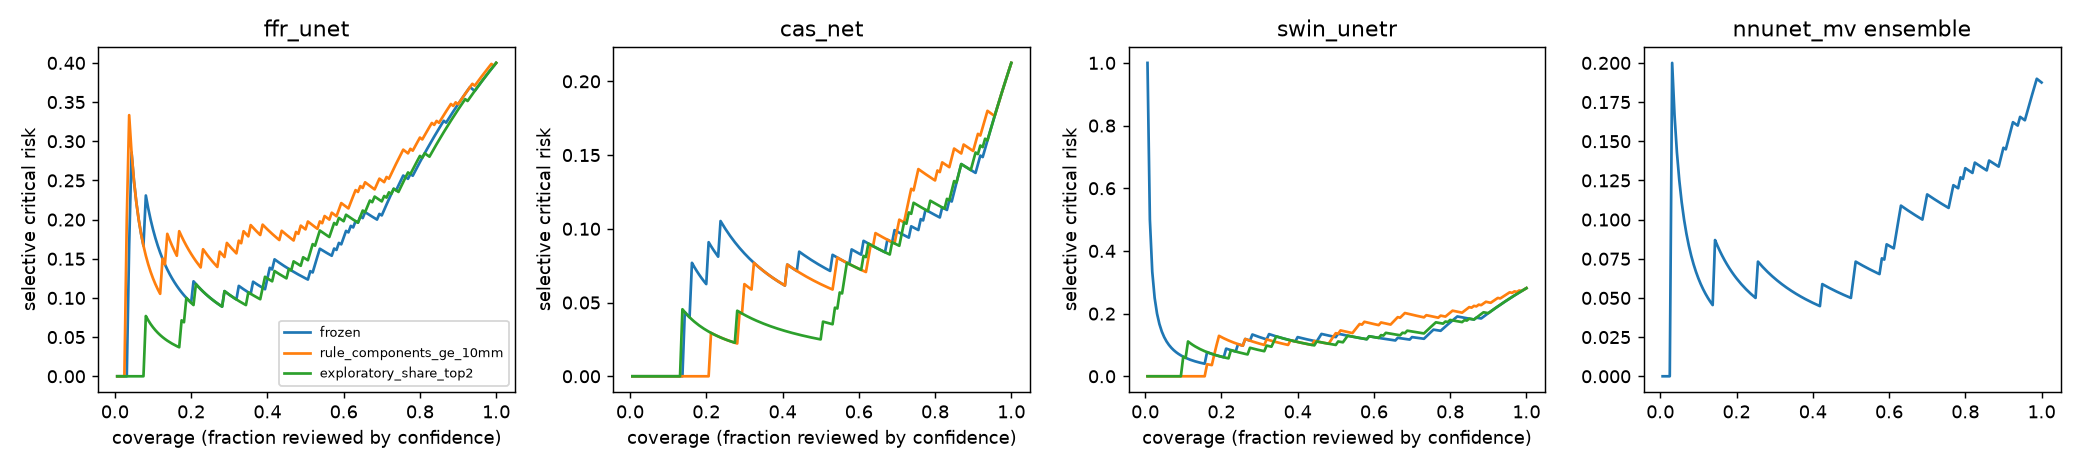
\includegraphics[width=\linewidth]{figures/risk_coverage.png}
\caption{Risk--coverage curves on the sealed test set: selective critical-failure risk against the fraction of reconstructions accepted, ordered by confidence. Frozen model (blue), pre-specified rule (orange), exploratory fragmentation feature (green), and ensemble agreement on nnU-Net majority-vote reconstructions (right).}
\label{fig:rc}
\end{figure}

\subsection{Pre-registered follow-up analyses}
Figure~\ref{fig:forest} summarises the follow-up analyses on the model-minus-rule difference.

\begin{figure}[t]
\centering
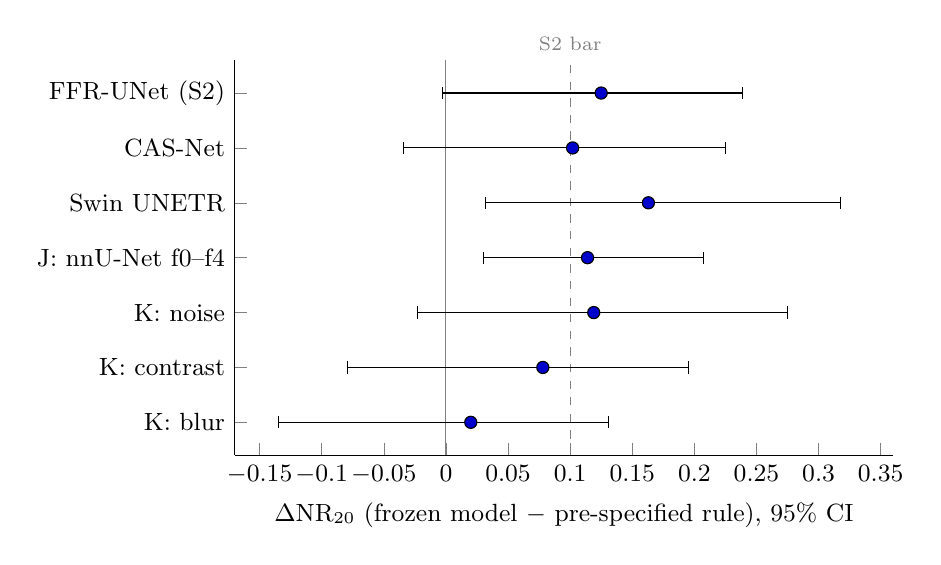
\begin{tikzpicture}
\begin{axis}[
  width=0.82\linewidth, height=6.6cm,
  xmin=-0.17, xmax=0.36,
  ymin=0.4, ymax=7.6,
  ytick={1,2,3,4,5,6,7},
  yticklabels={K: blur, K: contrast, K: noise, J: nnU-Net f0--f4, Swin UNETR, CAS-Net, FFR-UNet (S2)},
  yticklabel style={font=\small},
  xlabel={$\Delta\NR$ (frozen model $-$ pre-specified rule), 95\% CI},
  xlabel style={font=\small},
  xtick={-0.15,-0.10,-0.05,0,0.05,0.10,0.15,0.20,0.25,0.30,0.35},
  xticklabel style={font=\small,/pgf/number format/fixed,/pgf/number format/precision=2},
  extra x ticks={0.10},
  extra x tick style={grid=major, grid style={dashed,gray}},
  extra x tick labels={},
  axis lines*=left,
  clip=false,
]
\draw[gray] (axis cs:0,0.4) -- (axis cs:0,7.6);
\addplot+[only marks, mark=*, mark size=2.2pt, color=black,
  error bars/.cd, x dir=both, x explicit]
  coordinates {
  (0.125,7) -= (0.128,0) += (0.114,0)
  (0.102,6) -= (0.136,0) += (0.123,0)
  (0.163,5) -= (0.131,0) += (0.155,0)
  (0.114,4) -= (0.084,0) += (0.093,0)
  (0.119,3) -= (0.142,0) += (0.156,0)
  (0.078,2) -= (0.157,0) += (0.117,0)
  (0.020,1) -= (0.155,0) += (0.111,0)
  };
\node[font=\scriptsize, gray, anchor=south] at (axis cs:0.10,7.6) {S2 bar};
\end{axis}
\end{tikzpicture}
\caption{Model-minus-rule differences in normalised recall with patient-bootstrap 95\% CIs. FFR-UNet, CAS-Net and Swin UNETR: sealed test. J: mean over five nnU-Net folds (same 160 patients). K: CAS-Net on perturbed test CTs. The dashed line is the pre-registered $+10$\pp\ bar.}
\label{fig:forest}
\end{figure}

\paragraph{S2 diagnostics (Addendum M).} Among the 64 critical FFR-UNet units, 20 were caught by both rankers, 9 only by the model, 5 only by the rule and 30 by neither. The original bootstrap was reproduced exactly; at 20{,}000 resamples the CI was $[-0.7, +23.5]$\pp. An exact McNemar test \citep{mcnemar1947} on the discordant catches gave $p = 0.42$. A simulation that used the observed effect and discordance as truth (optimistic) gave only 40\% power to meet the S2 criterion at $n=160$, and 67\% even at $n = 480$. The criterion requires both an estimate $\geq +10$\pp\ and a lower bound $> 0$, and the true effect appears close to the bar. Under those conditions it is nearly unattainable at realistic sample sizes, which is consistent with the sample-size arguments of \citet{gibson2017power}.

\paragraph{Replication across nnU-Net folds (Addendum J).} We applied the frozen model, unchanged, to each of the five nnU-Net folds' test reconstructions, treating the folds as one correlated family. Per-fold differences were $+4.0$, $+17.1$, $+11.8$, $+15.6$ and $+8.6$\pp, with a mean of \textbf{$+11.4$\pp\ $[+3.0, +20.7]$}, which meets the S2 bar. The AUROC difference was positive in every fold. This is the same 160 patients, and the folds track a majority-vote result that had already been seen. It is evidence of consistency across reconstructions, not independent-patient validation. The exploratory fragmentation feature was within 0--7\pp\ of the model on every fold.

\paragraph{Acquisition-shift stress test (Addendum K).} We degraded the 160 test CTs in three pre-specified ways and re-ran CAS-Net on each: Gaussian noise raising the noise standard deviation by 50\%; isotropic Gaussian blur, $\sigma = 0.6$\,mm; and contrast compressed by 0.75 about the aortic median. Critical prevalence rose from 21\% to 22--29\%. The model's advantage over the rule was $+11.9$\pp\ under noise, $+7.8$\pp\ under contrast and $+2.0$\pp\ under blur, all with CIs including zero. Its AUROC advantage disappeared under all three. Every model input is derived from the predicted mask, and the aorta mask came from the unperturbed CT. The shrinking advantage therefore reflects a change in the segmenter's failure profile, not image features failing: the learned combination's increment over a single topology feature is not robust to shift.

\paragraph{Independent-lumen burden (Addendum L).} To probe label circularity, we built a failure measure without the taxonomy machinery: the fraction of the \emph{original} ImageCAS lumen, inside a 2\,mm band around the major vessels, that the prediction does not cover. The frozen score correlated with this measure (pooled Spearman 0.26 $[0.13, 0.37]$), including after regressing out the taxonomy burden (0.13 $[0.03, 0.22]$). Per segmenter, the association held for FFR-UNet, held only before adjustment for Swin UNETR, and was not significant for CAS-Net. The measure is dominated by a lumen-definition mismatch (mean value about 0.65 for every segmenter; see the next paragraph), so we treat this as weak support only.

\paragraph{Second-annotator relabelling (Addendum I, negative).} We planned to recompute the critical labels against the original ImageCAS masks as a second annotation. On validation, these masks covered a 2--6$\times$ larger lumen than ImageCAS-X and contained 80--99\% of it (median Dice 0.43), with identical grids and no orientation error. Relabelled prevalence was 0.93 against 0.13 (kappa 0.02). The two references encode different lumen definitions, so this analysis cannot test label robustness. We did not run it on the test set.

\subsection{Downstream consequences and negative findings}
Pooled over FFR-UNet, CAS-Net and Swin UNETR, vessels in flagged reconstructions had more severe-stenosis category flips than unflagged ones (2.1\% $[0.5, 4.3]$ vs 0.3\% $[0.0, 0.6]$; diameter-stenosis bands following CAD-RADS 2.0 \citep{cury2022cadrads}). They also had more vessels with reference-centerline coverage below 0.9 (17.2\% vs 9.1\%). These are geometric proxies computed from masks, not clinical outcomes.

Three planned components failed and are reported as negative results. (i) The synthetic-corruption CNN (M4) was uninformative on its own: corruptions of reference trees did not resemble real segmenter errors. (ii) A reduced-order 1D fractional-flow-reserve model was unstable to sub-voxel perturbations: the 95th percentile of the test--retest $|\Delta\mathrm{FFR}|$ was about 0.3, even with TEASAR centerlines and sub-voxel radii. This agrees with reports of high FFR-CT sensitivity to lumen uncertainty \citep{fernandez2024ffrct}, and we made no FFR claims. (iii) Uncertainty features (test-time-augmentation disagreement and entropy) added nothing to the graph features on development data.

\section{Discussion}
Label-free triage of coronary reconstructions works in the sense that matters operationally. Reviewing a fifth of the cases catches most of the critical failures that are catchable at that budget, and more than ensemble agreement (0.600 vs 0.500 on the same majority-vote reconstructions). Three findings limit what a learned model adds, however. First, the pre-registered superiority test over a simple rule failed narrowly, and the estimator diagnostics show it would be hard to pass at any realistic sample size, given an effect close to the bar. Second, an exploratory single feature, fragmentation of the predicted tree, matched the model. Third, the model's increment shrank under acquisition shift. The fold replication shows the increment is directionally consistent across reconstructions of the same patients.

For practice, this suggests starting with transparent topology features (component structure, ostium attachment) for coronary QC, and justifying learned combinations by replication on new patients and sites. It also explains why ensemble agreement underperformed here: fold disagreement measures uncertainty, while critical failures in coronary trees are often systematic and shared across folds.

\paragraph{Limitations.} All data come from one source cohort (ImageCAS); we found no openly available independent CCTA dataset with comparable lumen labels for external testing. The failure taxonomy is reference-based and was not defined or adjudicated by clinicians, and there is no reader study. The fold replication and stress test reuse the same 160 test patients. The pre-registration is self-maintained rather than in a public registry. The critical tier was motivated by label prevalence on two development segmenters' reconstructions, although no QA score was examined. Calibration was moderate, and conformal risk control did not give useful guarantees at this sample size.

\paragraph{Use of AI assistants.} The analysis code, experiment orchestration and manuscript drafts were produced with substantial assistance from AI coding and writing assistants (Anthropic Claude, OpenAI Codex, DeepSeek), working under the author's direction. The author directed the study, reviewed the analyses and results, and takes full responsibility for the content.

\paragraph{Acknowledgements.} Compute was provided by an AMD Developer Cloud credit (AMD Instinct MI300X). We thank the creators of ImageCAS and ImageCAS-X for making their data and models available.

\paragraph{Data and code.} ImageCAS and ImageCAS-X are available from their authors under their respective terms; this work redistributes no images or labels. Code, the frozen model hashes and the full pre-registration trail will be released with a later version of this preprint.

\bibliographystyle{plainnat}
\bibliography{refs}
\end{document}
